\section{Risultati}\label{sec:results}

Per l'analisi dei risultati noiseless, abbiamo utilizzato una configurazione con 
8 asset, un budget massimo pari a 5, una penalità impostata sul valore del budget, 
un rischio pari a 0.3 e 50 ripetizioni per ciascun algoritmo. 
La Figura~\ref{fig:noiseless-risultati-1} mostra rispettivamente la distribuzione 
delle selezioni effettuate dagli algoritmi QAOA, VQE e Exact Eigensolver.

L'algoritmo QAOA evidenzia una preferenza marcata per specifici asset, che vengono 
selezionati con una frequenza significativamente maggiore rispetto agli altri. 
Questo comportamento è legato alla natura parametrizzata dell'algoritmo e alla 
sensibilità verso i valori iniziali dei parametri scelti per l'ottimizzazione. 
Tuttavia, questa limitata capacità esplorativa può risultare in una perdita di 
soluzioni ottimali o in una convergenza verso configurazioni subottimali.

D'altra parte, il VQE mostra una distribuzione più variegata delle selezioni. 
La capacità dell'algoritmo di adattare i parametri dell'ansatz consente di 
esplorare con maggiore efficacia lo spazio delle soluzioni. Nonostante questa 
maggiore diversificazione, i risultati non sono sempre allineati con quelli 
ottimali, evidenziando che alcune incertezze permangono anche in questo caso.

L'Exact Eigensolver rappresenta la \textit{ground truth} del problema. Questo 
metodo fornisce sempre la soluzione esatta e ottimale del problema, servendo 
da riferimento principale per valutare la qualità dei risultati ottenuti con 
gli approcci approssimati. La sua precisione consente di identificare con 
certezza gli asset migliori da selezionare.

La Figura~\ref{fig:noiseless-risultati-2} confronta le distribuzioni delle 
selezioni dei tre algoritmi, evidenziando le principali differenze. Il QAOA 
tende a concentrare le sue scelte su un insieme ristretto di asset, 
confermando una minore capacità esplorativa rispetto al VQE, che riesce 
invece a bilanciare meglio esplorazione ed exploitazione.

Infine, la Figura~\ref{fig:noiseless-risultati-3} analizza la frequenza 
delle combinazioni di asset selezionate nei 50 esperimenti. Anche qui 
si nota come il QAOA presenti una concentrazione delle combinazioni 
selezionate, mentre il VQE esplora una maggiore varietà di configurazioni. 

\begin{figure}[ht!]
    \centering
    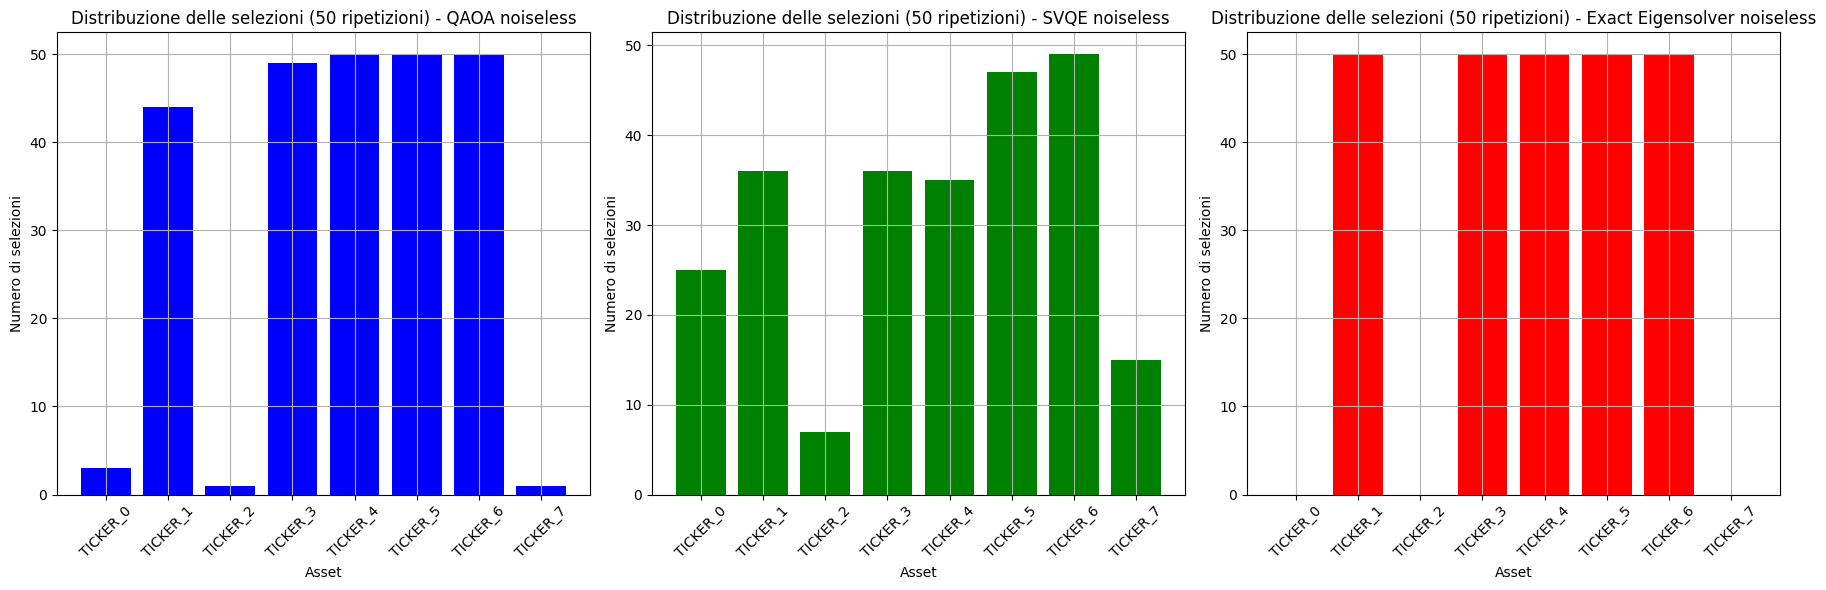
\includegraphics[width=0.99\textwidth]{images/risultati/noiseless-risultati-1.png}
    \caption{Distribuzione delle selezioni effettuate dagli algoritmi QAOA, VQE e Exact Eigensolver.}
    \label{fig:noiseless-risultati-1}
\end{figure}
\begin{figure}[ht!]
    \centering
    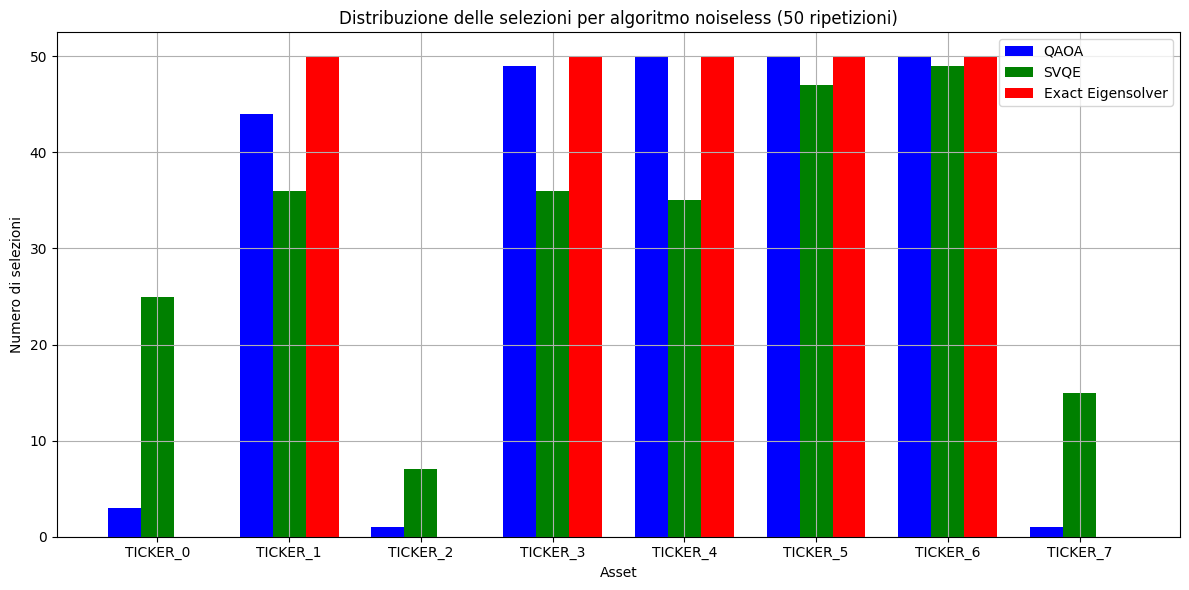
\includegraphics[width=0.99\textwidth]{images/risultati/noiseless-risultati-2.png}
    \caption{Distribuzione delle selezioni per algoritmo.}
    \label{fig:noiseless-risultati-2}
\end{figure}
\begin{figure}[ht!]
    \centering
    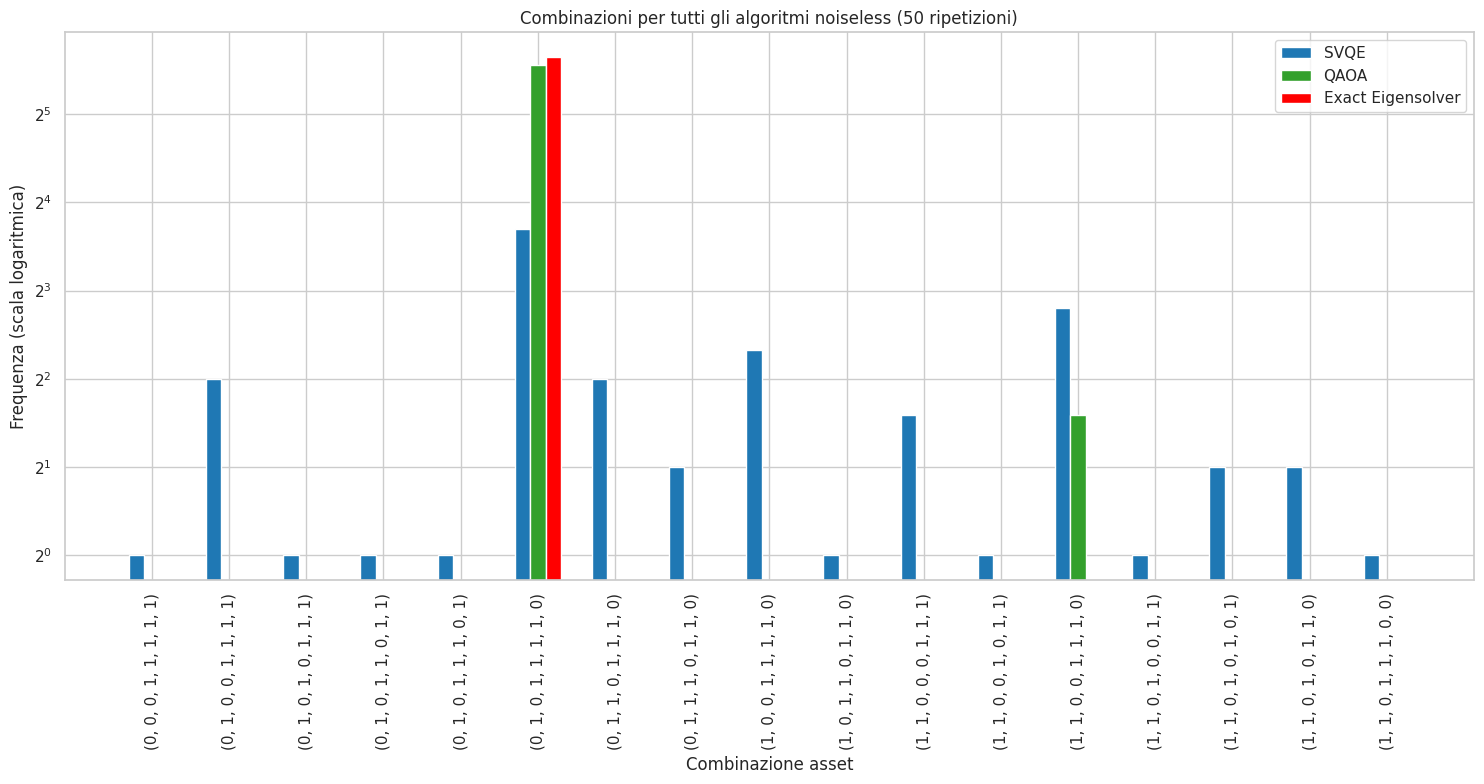
\includegraphics[width=0.99\textwidth]{images/risultati/noiseless-risultati-3.png}
    \caption{Frequenza delle combinazioni di asset selezionate nei 50 esperimenti.}
    \label{fig:noiseless-risultati-3}
\end{figure}


\subsection{Risultati Noisy}

Per l'analisi dei risultati noisy, abbiamo utilizzato la stessa configurazione 
di base con 8 asset, un budget massimo pari a 5, una penalità impostata sul valore 
del budget, un rischio pari a 0.3 e 50 ripetizioni per ciascun algoritmo. 
La Figura~\ref{fig:noisy-risultati-1} mostra rispettivamente la distribuzione 
delle selezioni effettuate dagli algoritmi QAOA e VQE in presenza di rumore.

L'algoritmo QAOA, in presenza di rumore, mostra una distribuzione delle selezioni 
ancora più concentrata rispetto alla versione noiseless. Questo comportamento 
è dovuto alla sensibilità dell'algoritmo ai rumori di decoerenza e di gate, 
che influenzano negativamente la capacità dell'algoritmo di esplorare lo spazio 
delle soluzioni. La presenza di rumore tende a far convergere l'algoritmo verso 
configurazioni subottimali, riducendo ulteriormente la diversificazione delle selezioni.

Il VQE, sebbene anch'esso influenzato dal rumore, riesce a mantenere una 
distribuzione delle selezioni più variegata rispetto al QAOA. La capacità 
dell'algoritmo di adattare i parametri dell'ansatz consente di mitigare 
parzialmente gli effetti del rumore, sebbene i risultati mostrino comunque 
una riduzione della qualità delle soluzioni rispetto alla versione noiseless.

La Figura~\ref{fig:noisy-risultati-2} confronta le distribuzioni delle selezioni 
dei due algoritmi in presenza di rumore, evidenziando le principali differenze. 
Il QAOA tende a concentrare le sue scelte su un insieme ancora più ristretto di asset 
rispetto alla versione noiseless, mentre il VQE riesce a mantenere una maggiore 
varietà nelle selezioni, sebbene con una qualità complessiva inferiore.

Infine, la Figura~\ref{fig:noisy-risultati-3} analizza la frequenza delle combinazioni 
di asset selezionate nei 50 esperimenti in presenza di rumore. Anche qui si nota come 
il QAOA presenti una concentrazione delle combinazioni selezionate, mentre il VQE 
esplora una maggiore varietà di configurazioni, sebbene con una frequenza ridotta 
rispetto alla versione noiseless.

\begin{figure}[ht!]
    \centering
    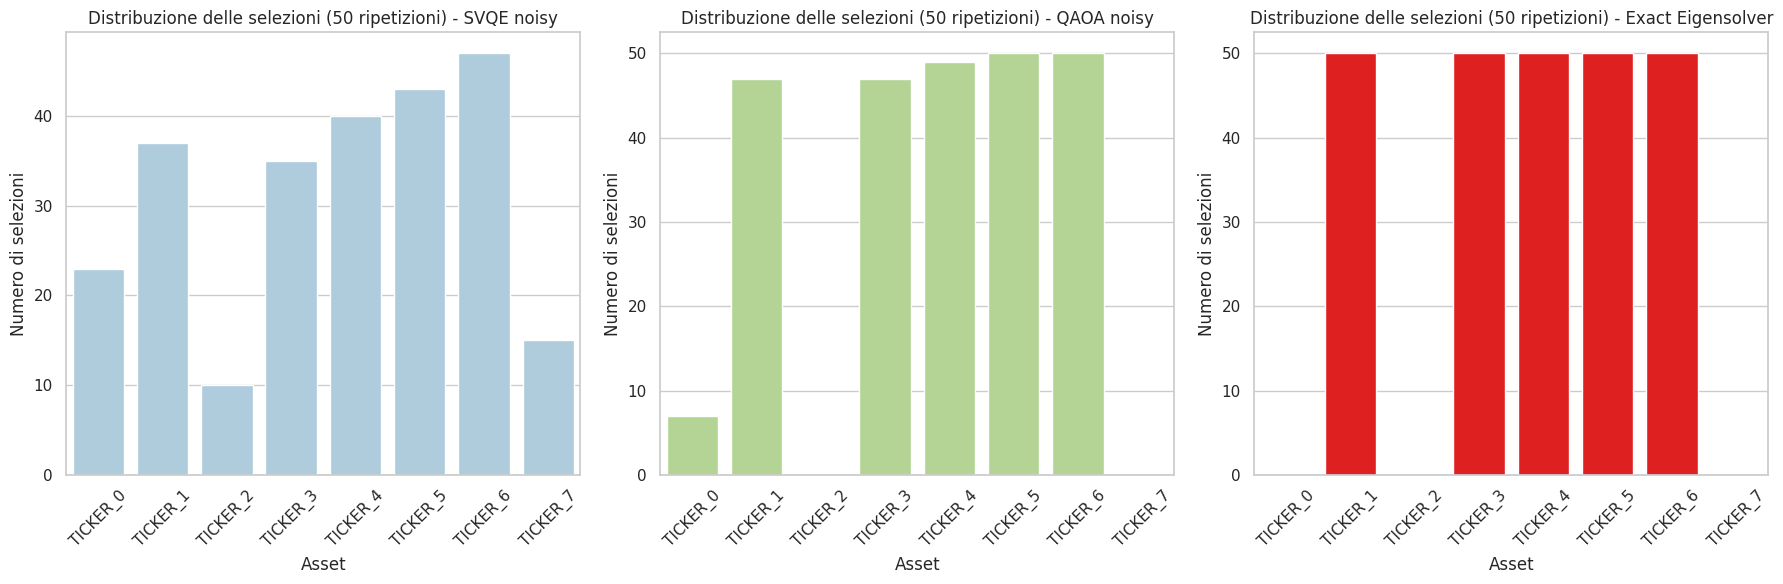
\includegraphics[width=0.99\textwidth]{images/risultati/noisy-risultati-1.png}
    \caption{Distribuzione delle selezioni effettuate dagli algoritmi QAOA e VQE in presenza di rumore.}
    \label{fig:noisy-risultati-1}
\end{figure}
\begin{figure}[ht!]
    \centering
    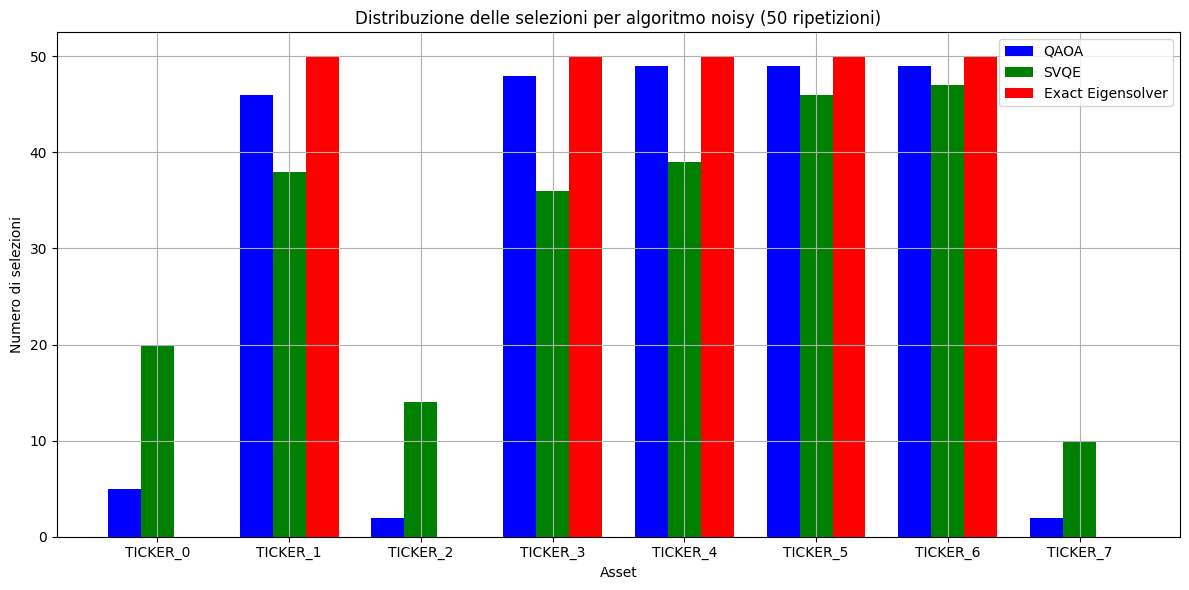
\includegraphics[width=0.99\textwidth]{images/risultati/noisy-risultati-2.png}
    \caption{Distribuzione delle selezioni per algoritmo in presenza di rumore.}
    \label{fig:noisy-risultati-2}
\end{figure}
\begin{figure}[ht!]
    \centering
    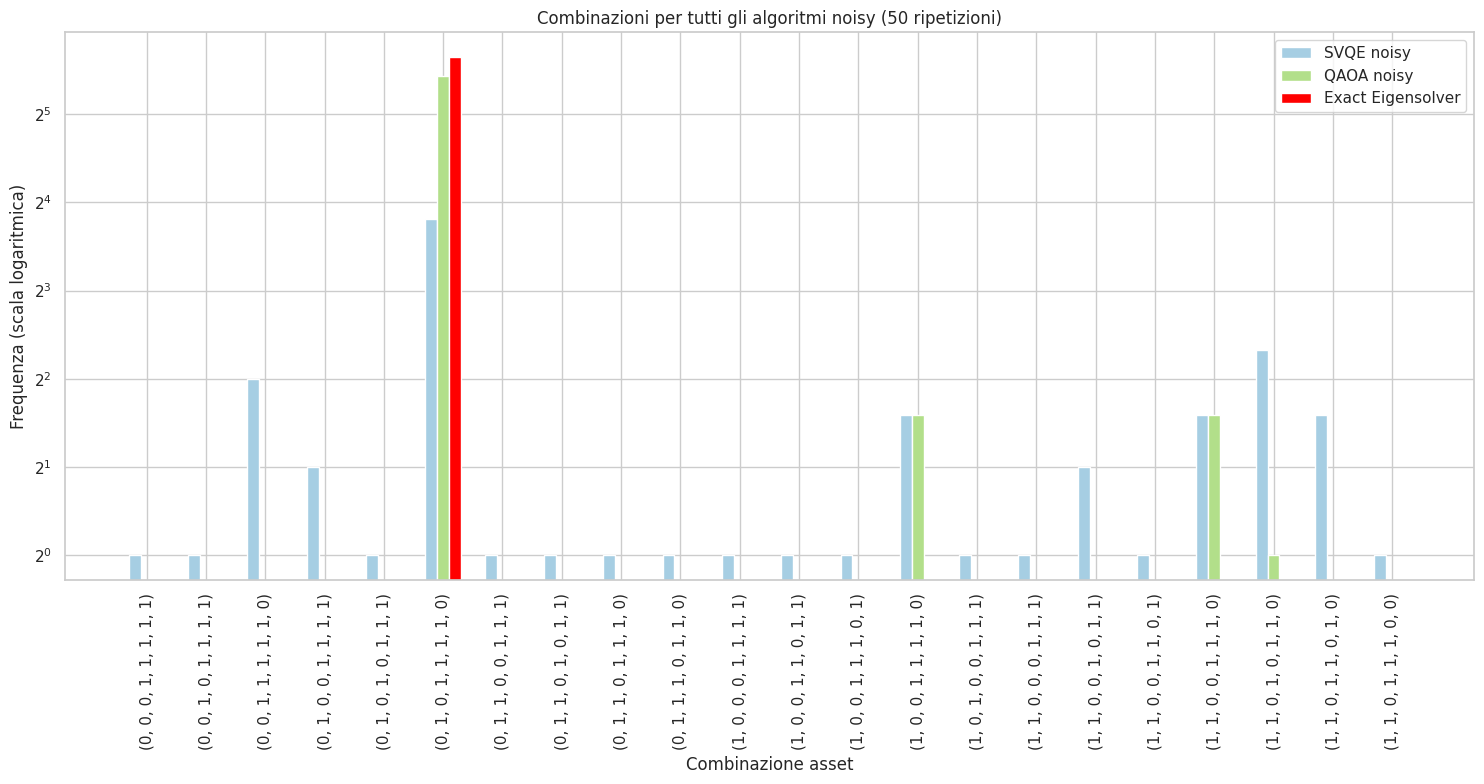
\includegraphics[width=0.99\textwidth]{images/risultati/noisy-risultati-3.png}
    \caption{Frequenza delle combinazioni di asset selezionate nei 50 esperimenti in presenza di rumore.}
    \label{fig:noisy-risultati-3}
\end{figure}


\paragraph{Confronto algoritmi (noiseless vs noisy)}
Infine, confrontiamo i risultati ottenuti dagli algoritmi QAOA e VQE in 
condizioni noiseless e noisy. Questo confronto ci permette di valutare l'impatto 
del rumore sulle prestazioni degli algoritmi e sulla qualità delle soluzioni ottenute.

La Figura~\ref{fig:confronto-svqe-noiseless-noisy} mostra il confronto delle combinazioni selezionate 
dall'algoritmo VQE in condizioni noiseless e noisy. Si può osservare che, in presenza 
di rumore, l'algoritmo VQE tende a selezionare un insieme più variegato di combinazioni 
rispetto alla versione noiseless. Questo comportamento è dovuto alla capacità 
dell'algoritmo di adattare i parametri dell'ansatz, che consente di esplorare con 
maggiore efficacia lo spazio delle soluzioni anche in presenza di rumore. Tuttavia, 
la qualità complessiva delle soluzioni ottenute dal VQE risulta inferiore rispetto a 
quella del QAOA, evidenziando una maggiore difficoltà nell'ottenere una scelta ottimale 
delle soluzioni in presenza di rumore.

La Figura~\ref{fig:confronto-qaoa-noiseless-noisy} mostra il confronto delle combinazioni selezionate 
dall'algoritmo QAOA in condizioni noiseless e noisy. Anche in questo caso, si nota un 
insieme più variegato di soluzioni in presenza di rumore, ma comunque non ci si 
allontana di molto dalla soluzione ottimale. L'algoritmo QAOA, nonostante la presenza 
di rumore, riesce a mantenere una buona qualità delle soluzioni, dimostrando una 
maggiore robustezza rispetto al VQE.

\begin{figure}[ht!]
    \centering
    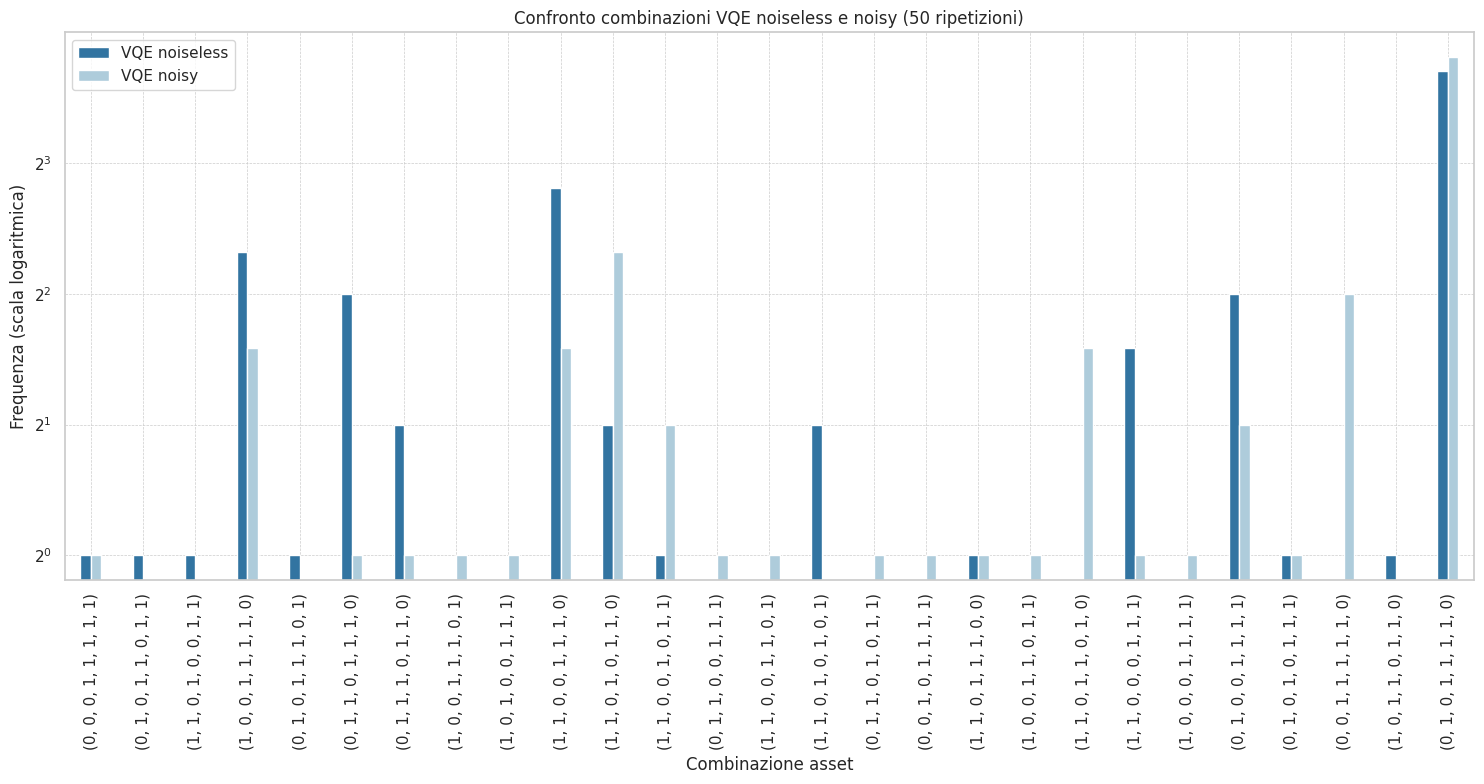
\includegraphics[width=0.99\textwidth]{images/risultati/confronto-svqe.png}
    \caption{Confronto delle combinazioni selezionate dall'algoritmo VQE in condizioni noiseless e noisy.}
    \label{fig:confronto-svqe-noiseless-noisy}
\end{figure}

\begin{figure}[ht!]
    \centering
    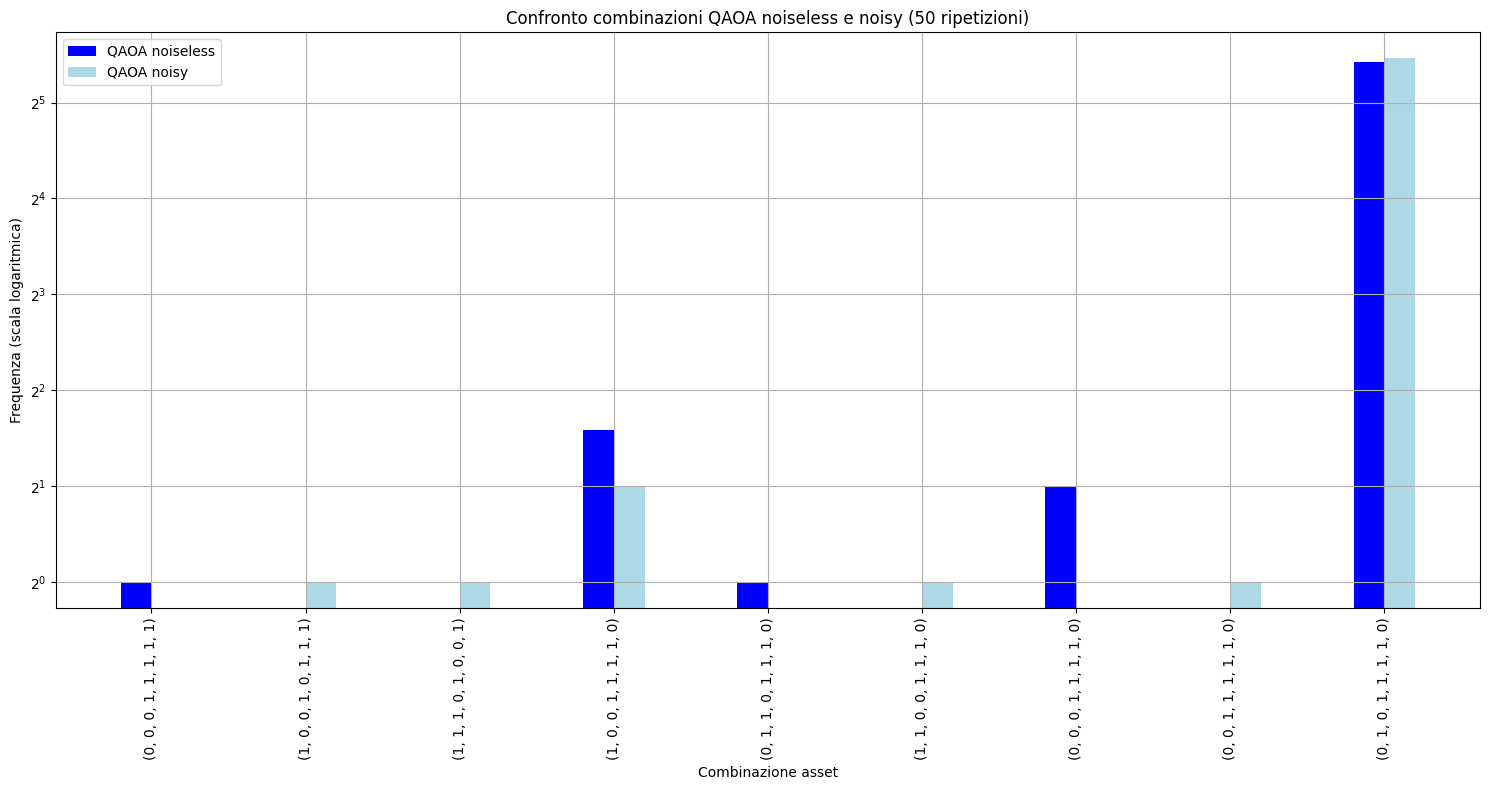
\includegraphics[width=0.99\textwidth]{images/risultati/confronto-qaoa.png}
    \caption{Confronto delle combinazioni selezionate dall'algoritmo QAOA in condizioni noiseless e noisy.}
    \label{fig:confronto-qaoa-noiseless-noisy}
\end{figure}


